\documentclass[11pt]{article}
\usepackage{geometry}                
\geometry{letterpaper}                 
\usepackage[parfill]{parskip}        
\usepackage{graphicx}
\usepackage{amssymb}
\usepackage{amsmath}
\usepackage{epstopdf}
\usepackage{verbatim}
\usepackage{float}
\usepackage{enumerate}
\usepackage{hyperref}
\usepackage[utf8]{inputenc}
\usepackage[T1]{fontenc}
\usepackage{polynom}
\DeclareGraphicsRule{.tif}{png}{.png}{`convert #1 `dirname #1`/`basename #1 .tif`.png}
\usepackage{color}
\usepackage{textcomp}
\definecolor{listinggray}{gray}{0.9}
\definecolor{lbcolor}{rgb}{1,1,1}


\begin{document}
Solutions for homework 4, problems \#2,3

\section*{Problem 2, 3.25 O\&S 3rd Ed.}

Sketch each of the following sequences and determine their z-transforms, including the region of convergence.

\subsection*{(a)}

$a[n] = \sum\limits_{k=-\infty}^\infty \delta[n-4k]$

\begin{eqnarray*}
A(z) &=& \sum_{n=-\infty}^\infty \sum\limits_{k=-\infty}^\infty \delta[n-4k] z^{-n} \\
&=& \sum\limits_{k=-\infty}^\infty \left(\sum_{n=-\infty}^\infty  \delta[n-4k] z^{-n}\right) \\
\text{from the sifting property,} &=& \sum\limits_{k=-\infty}^\infty z^{-4k} \\
&=& \sum\limits_{k=0}^\infty (z^{-4})^k + \sum\limits_{k=-\infty}^{-1} (z^{-4})^k \\
&=& \underbrace{\sum\limits_{k=0}^\infty (z^{-4})^k}_\alpha + \underbrace{\sum\limits_{k=1}^{\infty} (z^{4})^k}_\beta \\
\end{eqnarray*}

Note that $\alpha$ converges only if $|z^{-4}|<1$ and $\beta$ converges only if $|z^4|<1$. There is no complex number $z$ that satisfies both of these conditions. Since the ROC of $A(z)$ is the intersection of the ROC of $\alpha$ $\cap$ ROC of $\beta$, ROC of $A(z)$ is empty, $\{\}$.

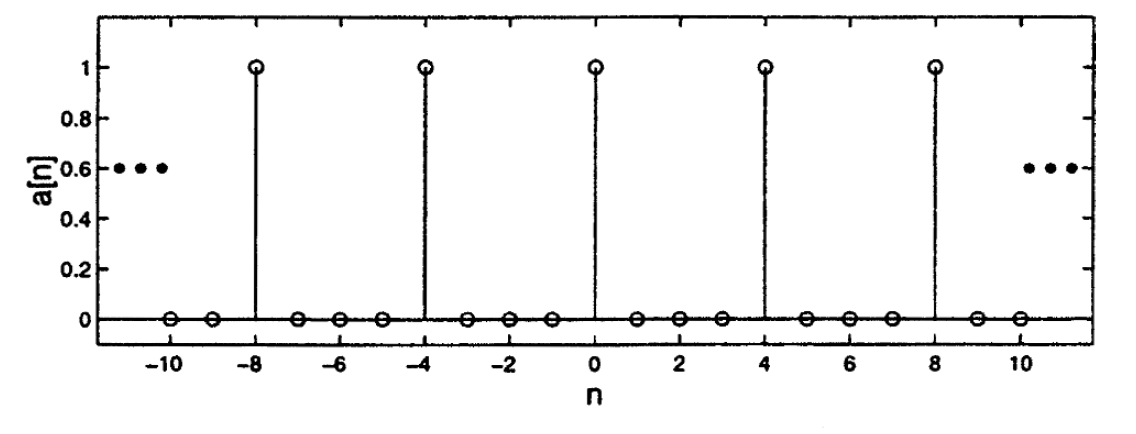
\includegraphics[width=0.9\textwidth]{Soln4/p2a.png} 

\subsection*{(b)}

$b[n] = \frac{1}{2}\left[ e^{j\pi n} + cos\left(\frac{\pi}{2}n\right)+sin\left(\frac{\pi}{2}+2\pi n\right)\right] u[n]$

First, let us simplify $x[n]$.

\begin{eqnarray*}
b[n] &=& \frac{1}{2}\left[ e^{j\pi n} + cos\left(\frac{\pi}{2}n\right)+sin\left(\frac{\pi}{2}+2\pi n\right)\right] u[n] \\
&=& \frac{1}{2}\left[ (-1)^n + cos\left(\frac{\pi}{2}n\right)+sin\left(\frac{\pi}{2}\right)\right] u[n] \\
&=& \frac{1}{2}\left[ (-1)^n + cos\left(\frac{\pi}{2}n\right)+1 \right] u[n] \\
&=& \begin{cases}
\frac{3}{2}, & n=4k, k\geq 0 \\
\frac{1}{2}, & n=4k+2, k\geq 0 \\
0, & otherwise
\end{cases}
\end{eqnarray*}

\begin{eqnarray*}
B(z) &=& \sum_{n=-\infty}^\infty b[n] z^{-n} \\
&=& \sum_{\substack{n=-\infty \\ n=4k\geq 0}}^\infty b[n] z^{-n} + \sum_{\substack{n=-\infty \\ n=2+4k \geq 0}}^\infty b[n] z^{-n} + \sum_{\substack{n=-\infty \\ n \text{ odd or } n < 0}}^\infty b[n] z^{-n} \\
&=& \sum_{\substack{n=-\infty \\ n=4k\geq 0}}^\infty \frac{3}{2} z^{-n} + \sum_{\substack{n=-\infty \\ n=2+4k \geq 0}}^\infty \frac{1}{2} z^{-n} + \sum_{\substack{n=-\infty \\ n \text{ odd or } n < 0}}^\infty 0 \cdot z^{-n} \\
&=& \sum_{k=0}^\infty \frac{3}{2} z^{-4k} + \sum_{k=0}^\infty \frac{1}{2} z^{-(2+4k)}  \\
&=& \left(\frac{3}{2} + \frac{1}{2}z^{-2} \right) \sum_{k=0}^\infty (z^{-4})^k  \\
&=& \left(\frac{3}{2} + \frac{1}{2}z^{-2} \right) \left(\frac{1}{1-z^{-4}} \right) \text{ for }|z^{-4}| < 1 \text{, or equivalently } |z|>1\\
&=& \frac{\frac{3}{2}+\frac{1}{2}z^{-2}}{1-z^{-1}} \text{ with ROC } |z| > 1\\
\end{eqnarray*}

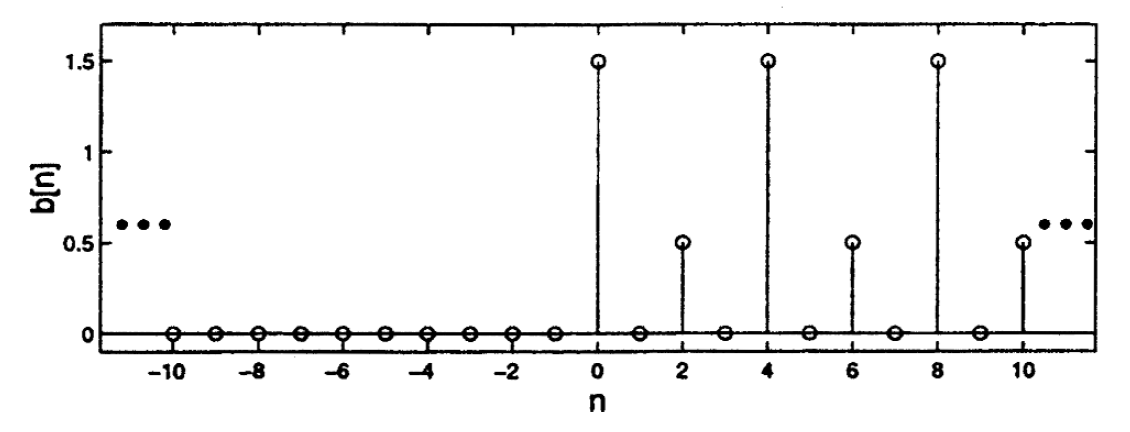
\includegraphics[width=0.9\textwidth]{Soln4/p2b.png} 

\section*{Problem 3, 3.31 O\&S 3rd Ed.}

Determine the inverse z-transform of each of the following. In Parts (a)-(c), use the methods specified. In Part (d), use any method you prefer.

\subsection*{(a) Long division:}

$x[n]$ is right-sided and $X(z) = \frac{1-\frac{1}{3}z^{-1}}{1+\frac{1}{3}z^{-1}}$

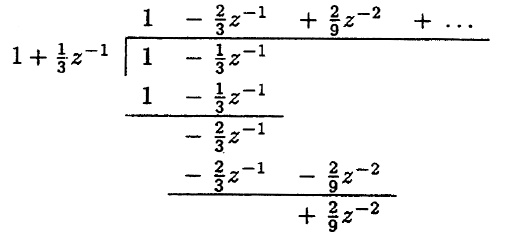
\includegraphics[width=0.5\textwidth]{Soln4/p3_longdivision.png} 

$1-\frac{2}{3}z^{-1}+\frac{2}{9}z^{-2}-\frac{2}{27}z^{-3}+\cdots = 2\left(1-\frac{1}{3}z^{-1}+\frac{1}{9}z^{-2}-\frac{1}{27}z^{-3}+\cdots\right) -1$

So we can take the inverse z-transform by inspection:

$x[n] = 2\{\underline{1},-\frac{1}{3},\frac{1}{9},-\frac{1}{27},\ldots\} - \{\underline{1},0,0,\ldots\} = 2\left(-\frac{1}{3}\right)^n u[n] - \delta[n]$

\subsection*{(b) Partial fraction:}

$X(z) = \frac{3}{z-\frac{1}{4}-\frac{1}{8}z^{-1}}$ and $x[n]$ is stable

First, we factor to find the denominator terms for the partial fraction expansion:
$X(z) = \frac{3}{z-\frac{1}{4}-\frac{1}{8}z^{-1}} = \frac{3z^{-1}}{1-\frac{1}{4}z^{-1}-\frac{1}{8}z^{-2}} = \frac{3z^{-1}}{(1-\frac{1}{2}z^{-1})(1+\frac{1}{4}z^{-1})}$

So now we know that it can be written in the form $X(z) = \frac{A_1}{1-\frac{1}{2}z^{-1}}+\frac{A_2}{1+\frac{1}{4}z^{-1}}$. To find $A_1$ and $A_2$, we use Equation 3.41:

$A_1 = (1-\frac{1}{2}z^{-1})\left(\frac{3z^{-1}}{(1-\frac{1}{2}z^{-1})(1+\frac{1}{4}z^{-1})}\right)\bigg|_{z=1/2}=\frac{3z^{-1}}{1+\frac{1}{4}z^{-1}}\bigg|_{z=1/2} = \frac{6}{1+\frac{1}{2}} = 4$

$A_2 = (1+\frac{1}{4}z^{-1})\left(\frac{3z^{-1}}{(1-\frac{1}{2}z^{-1})(1+\frac{1}{4}z^{-1})}\right)\bigg|_{z=-1/4} = \frac{3z^{-1}}{1-\frac{1}{2}z^{-1}}\bigg|_{z=-1/4} = \frac{-12}{1+2} = -4$

Thus, $X(z) = \frac{4}{1-\frac{1}{2}z^{-1}}+\frac{-4}{1+\frac{1}{4}z^{-1}}$

Since $x[n]$ is stable, the ROC must include the unit circle. It also has poles at $\frac{1}{2}$ and $-\frac{1}{4}$, so the ROC must be $|z|>\frac{1}{2}$, and $x[n]$ must be causal (or right-sided).

Therefore, $x[n]=4\left(\frac{1}{2}\right)^nu[n]-4\left(-\frac{1}{4}\right)^n u[n]$ 


\subsection*{(c) Power series:}
$X(z) = ln(1-4z)$ and $|z|<\frac{1}{4}$

Using the formula on page 117 (also covered in lecture), $X(z) = ln(1-4z) = \sum\limits_{n=1}^\infty \frac{(-1)^{n+1}(-4z)^n}{n} = - \sum\limits_{n=1}^\infty \frac{(4z)^n}{n}$ 

Note that the above series converges only if $|-4z|<1$, but this is consistent with $|z|<\frac{1}{4}$.

Let $m=-n$ and let's change variables. $X(z) = \sum\limits_{m=-\infty}^{-1}\frac{4^{-m}}{m}z^{-m}$ 

Hey, this looks like the definition of the z-transform. Since we know $x[n]$ is left-sided, we have $X(z) = \sum\limits_{m=-\infty}^{\infty}\left(\frac{4^{-m}}{m}u[-m-1]\right)z^{-m}$, and by inspection we arrive at $x[n]=\frac{1}{n}(4)^{-n}u[-n-1]$.


\subsection*{(d)}
$X(z) = \frac{1}{1-\frac{1}{3}z^{-3}}$, $|z|>(3)^{-1/3}$

We choose to analyze this with long division:

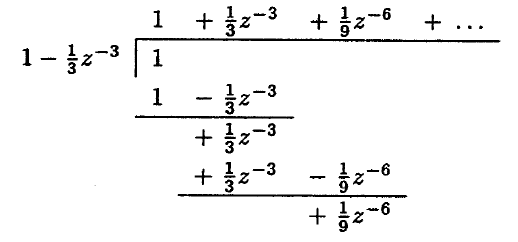
\includegraphics[width=0.5\textwidth]{Soln4/p3d.png} 

Because the ROC extends outward, we know that $x[n]$ is right-sided. By inspection we see that this is $x[n] = \begin{cases}
\left(\frac{1}{3}\right)^\frac{n}{3}, & n = 0,3,6,\ldots \\
0, & otherwise
\end{cases}$


\end{document}